\begin{center}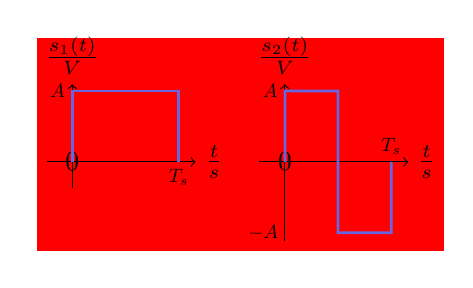
\begin{tikzpicture}[scale=0.9]
\fill[red]  (-0.5,1.75) rectangle (5.25,-1.25);

\node (null2) at (3,0) {$0$};
\node (startY2) at (3,-1.25) {};
\node (endY2) at (3,1.5) {$\frac{s_2(t)}{V}$};
\node (startX2) at (2.5,0) {};
\node (endX2) at (5,0) {$\frac{t}{s}$};
\draw [->] (startX2) edge (endX2);
\draw [->] (startY2) edge (endY2);

\node (null) at (0,0) {$0$};
\node (startY) at (0,-0.5) {};
\node (endY) at (0,1.5) {$\frac{s_1(t)}{V}$};
\node (startX) at (-0.5,0) {};
\node (endX) at (2,0) {$\frac{t}{s}$};
\draw [->] (startX) edge (endX);
\draw [->] (startY) edge (endY);
\draw[blue!80!black!60, line width=1pt] (0,0) -- (0,1) node[left,black,scale=0.7] {$A$} -- (1.5,1) -- (1.5,0) node[below,black,scale=0.7] {$T_s$};

\draw[blue!80!black!60, line width=1pt] (null2.center) -- (3,1) node[left,black,scale=0.7] {$A$} -- (3.75,1) -- (3.75,-1) -- (4.5,-1) -- (4.5,0) node[above,black,scale=0.7] {$T_s$};
\node[left,scale=0.7] at (3,-1) {$-A$};
\end{tikzpicture}\end{center}